\documentclass[12pt,english]{article}
\usepackage[a4paper,bindingoffset=0.2in,%
            left=1in,right=1in,top=1in,bottom=1in,%
            footskip=.25in]{geometry}
\usepackage{amsmath}
\usepackage{graphicx}
\usepackage{listings}
\usepackage{color}

\definecolor{dkgreen}{rgb}{0,0.6,0}
\definecolor{gray}{rgb}{0.5,0.5,0.5}
\definecolor{mauve}{rgb}{0.58,0,0.82}

\lstset{frame=tb,
  language=Matlab,
  aboveskip=3mm,
  belowskip=3mm,
  showstringspaces=false,
  columns=flexible,
  basicstyle={\small\ttfamily},
  numbers=none,
  numberstyle=\tiny\color{gray},
  keywordstyle=\color{blue},
  commentstyle=\color{dkgreen},
  stringstyle=\color{mauve},
  breaklines=true,
  breakatwhitespace=true,
  tabsize=3
}

\graphicspath{ {./figures/} }

\title{Proiect SNC}
\date{2019\\ Octombrie}
\author{Pangratie Andrei - 342 B3}

\begin{document}

\maketitle
\newpage

\tableofcontents
\newpage

\section { Pregatire experiment identificare }
\subsection { Platforma Laborator 3 de citit }
\subsection { Se studiaza fisa de activități }
\subsection { nu exista in cerinta 1.3 ??? }
\subsubsection { Grafice Raspuns indicial (comanda si iesire) }
\begin{center}
  \fbox{ 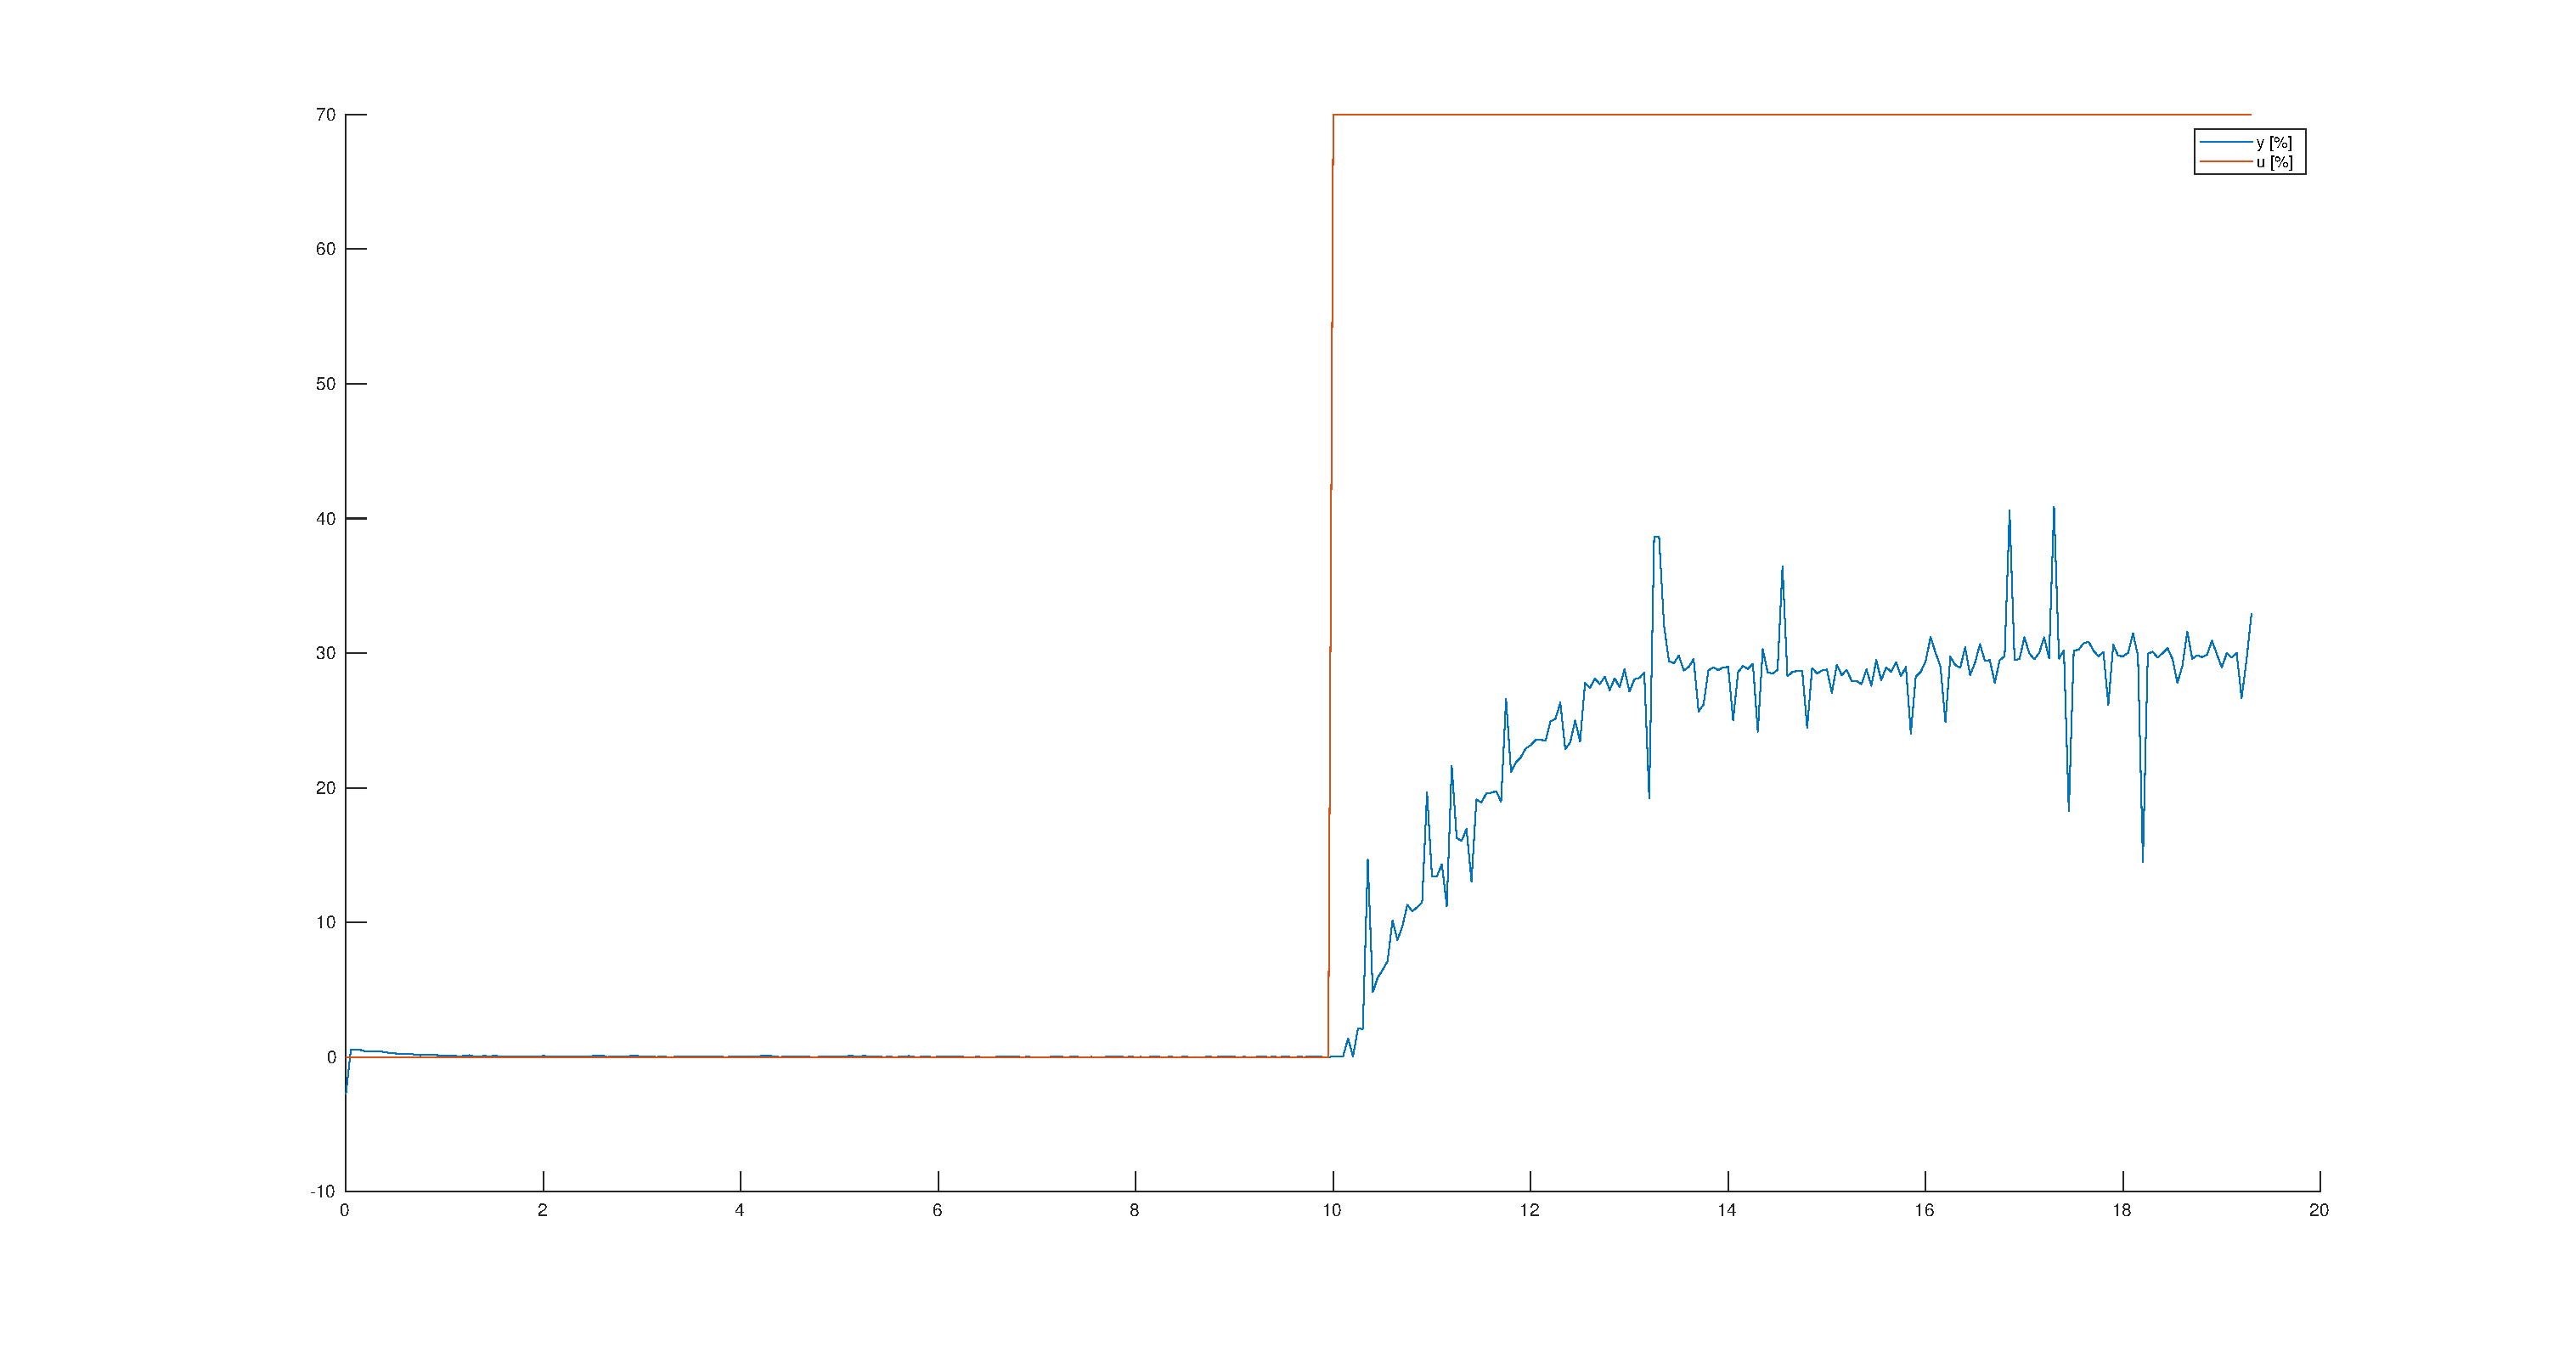
\includegraphics[width=1\textwidth]{1_3_1.eps}}
\end{center}

\subsubsection { [1p] Comentarii referitor grafice obtinute (scris/audio/video - la alegere) }
\subsection { Datele masurate salvate (link ?) }
\subsection { Caracteristici proces }
\subsection { Rezolvare Aplicatii Lab 3 }

\section { REALIZARE SI ANALIZA EXPERIMENT IDENTIFICARE }
\subsection { Expresia Matlab de generare a semnalului SPAB }
\subsection { [2p] Caracteristici semnal SPAB de intrare }
\subsection { [3p] Afisare spectrul semnal SPAB de intrare }
\subsection { [1p] Observatii asupra semnalului SPAB generat }
\subsection { Realizare experiment identificare (conform instructiunilor din laborator) }
\subsection { Fisier rezultate identificare (link). Fiserul este de tip .mat in care este salvat o structura tip iddata care contine intrarea, iesirea si configurarea unor parametri (exp Te). }
\subsection { [3p] Afisare spectrul semnal SPAB de iesire (achizitionat) }
\subsection { [1p] Observatii asupra semnalului achizitonat }

\section { IDENTIFICARE SI VALIDARE MODEL MATLAB }
\subsection { Platforma laborator 4 - citită                                  }
\subsection { [2p+1p+2p] Rezolvare Aplicatii Lab 4 }
\subsection { Filtrare semnale achiziționate in urma experimentului de identificare. }
\subsubsection { Functii Matlab apelate pentru filtrari: }
\subsubsection { [2p] Spectru semnale filtrate: }
\subsubsection { [1p] Comentarii asupra spectrului }
a
\subsection { Seturile de date de identificare Matlab - iddata pentru identificare si validare. }
b
\subsubsection { eData  (upload) }
c
\subsubsection { vData  (upload) }
d
\subsection { [2p] Estimarea complexității model ARX }
e
\subsubsection { Utilizare functie advice: ................. }
\subsubsection { Utilizare functie delayest: ................. }
\subsubsection { Estimare complexitate model ARX }
\subsection { Identificare model ARX }
\subsubsection { Descriere model obținut (structură, coeficienți, etc) }
\subsubsection { Valorile funcțiilor criteriu }
\subsubsection { Figurile obținute in urma validării ( resid \& compare) (vezi App Laborator 4) }
\subsection { [3p] Identificare model ARMAX }
\subsubsection { Descriere model obținut (structură, coeficienți, etc) }
\subsubsection { Valorile funcțiilor criteriu }
\subsubsection { Figurile obținute in urma validării ( resid \& compare) (vezi App Laborator 4) }
\subsection { [3p] Identificare model BJ }
\subsubsection { Descriere model ales (structură, coeficienți, etc) }
\subsubsection { Valorile funcțiilor criteriu }
\subsubsection { Figurile obținute in urma validării ( resid \& compare) (vezi App Laborator 4) }
\subsection { [3p] Identificare model OE }
\subsubsection { Descriere model ales (structură, coeficienți, etc) }
\subsubsection { Valorile funcțiilor criteriu }
\subsubsection { Figurile obținute in urma validării ( resid \& compare) (vezi App Laborator 4) }
\subsection { Alegere Model Final Matlab }
\subsubsection { Descriere model ales (structură, coeficienți, etc) }
\subsubsection { Valorile funcțiilor criteriu }
\subsubsection { Figurile obținute în urma validării (resid \& compare) }
\subsubsection { [1p] Studiul stabilității sistemului: ........... }
\subsubsection { Modelul Matlab ales încărcat este disponibil ?aici?. }
\subsubsection { Comentarii/Observații }

\section { MODELARE SI IDENTIFICARE FOLOSIND WIMPIM }
a
\subsection {4.1. [1p] Pregătire date inițiale WINPIM. Fisierul txt obtinut (upload) }
\subsection {4.2. [1p] Incarcare fisier in WinPIM si specificare perioada de esantionare }
\subsection {4.3. [1p] Aplicare filtrare set de date (eliminarea componentei continue) }
\subsection {4.4. [1p] Estimarea comlexitatii}
\subsection {4.5. [5p]  Identificare si validare modele }
\subsection {4.6. [1p] Modelul ales este anexat aici (BXY.mod) }
\subsection {4.7. [2p] Simulare model ales WinPIM si simulare model ales Matlab. }
\subsection {4.8. [2p]  Graficele simularilor sunt disponibile aici .  }
\subsection {4.9. Modelul final ales pentru continuarea proiectului este: }

\section { CALCUL REGULATOR RST-1, SIMULARE SI VALIDARE }
a
\subsection {5.1. Platforma laborator 6 - citită }
\subsection {5.2.  Obiective de reglare impuse  : }
\subsection {5.3. Pulsatia naturala si atenuarea echivalente cu obiectivele de reglare impuse: }
\subsection {5.4.[2p] Polii dominanti discreti impusi ca urmare a obiectivelor de reglare: }
\subsection {5.5. [2p] Specificare polinom P: }
\subsection {5.6. [2p] Grade polinoame ecuatia Sylvester }
\subsection {5.7. [2p]  Matricea M asociata : }
\subsection {5.8. [1p] Solutia ecuatiei}
\subsection {5.9. [3p] Pentru ca sistemul sa ofere timp de raspuns minim si suprareglaj < 5\% se aleg: }
\subsection {5.10. [4p]  Simulare sistem in bucla inchisa (comanda, referinta, iesirea), in conditii de perturbatii treapta (25\% amplitudine) aplicate dupa stabilizarea sistemului fata de referinta. Graficele sunt prezentate aici: }
\subsection {5.11. [1p] Observatii legate de rezultatele obtinute: }
\subsection {5.12. [1p] Specificare polinom P: }
\subsection {5.13 [1p] Grade polinoame ecuatia Sylvester }
\subsection {5.14. [2p]  Matricea M asociata : }
\subsection {5.15. [1p] Solutia ecuatiei}
\subsection {5.16. [2p]  Simulare sistem in bucla inchisa (comanda, referinta, iesirea), in conditii de perturbatii treapta (25\% amplitudine) aplicate dupa stabilizarea sistemului fata de referinta. Graficele sunt prezentate aici: }
\subsection {5.17. [1p] Observatii legate de rezultatele obtinute: }

\section { PROIECTARE REGULATOR RST-1 - WINPIM }
a
\subsection {6.1. Specificare performante in urmarire respectiv in reglare: }
\subsection {6.2. Pentru regulatorul calculat folosind metoda Pole Placement, cu integrator, polinoamele R,S,T sunt: }
\subsection {6.3. Fisierul WinPim cu regulator si model este aici. }
\subsection {6.4. Simulare sistem in bucla inchisa (comanda, referinta, iesirea), in conditii de perturbatii treapta (25\% amplitudine) aplicate dupa stabilizarea sistemului fata de referinta. Graficele sunt prezentate aici: }
\subsection {6.5. Observatii legate de rezultatele obtinute: }

\section { EVALUARE EXPERIMENTALA REGULATOR RST-1 }
a
\subsection { 7.1. Evaluare performante pe sistemul real. }
\subsubsection { Se alege referinta r(t) = ….  a.i. u(t) stationar sa fie egal cu u0. Pentru aceasta referinta s-a stimulat sistemul si s-a aplicat si o perturbatie cand a ajuns in regimul stationar de cca.\%}
\subsubsection { Rezultatul simularii se afla in imaginea de mai jos: }
\subsubsection { [2p] Alegand o alta referinta raspunsul sistemului este capturat in figura de mai jos: }
\subsection { 7.2. Performantele se regasesc rezumate in tabelul urmator }
\subsection { 7.3. Comentarii privind calitatea solutiei obtinute vs specificatiile impuse: }

\section { CALCUL REGULATOR RST-2, SIMULARE SI VALIDARE }
a
\subsection { 8.1. Platforma laborator 8 - citită }
\subsection { 8.2. [2p] Regulatorul RST 1 si-a indeplinit sau nu performantele impuse ?  Daca nu, ce masuri se iau (ce specificatii noi se impun fata de primul design ) ? }
\subsection { 8.3. [4p] Regulatorul RST 1 indeplineste marginile standard de robustete (se pot verifica cu aplicatia WinPIM)?   Figura cu functia de sensibilitate si template este furnizata aici. }
\subsection { 8.4. [4p] In cazul in care regulatorul a trebuit recalculat acesta este descris de polinoamele: }
\subsection { 8.5. [2p] Rezultatele in simulare sunt furnizate in figura urmatoare: }
\subsection { 8.6. [2p] Functia de sensibilitate a noii solutii: }

\section { Evaluare Experimentala Regulator RST-2 }
a
\subsection { 9.1. [3p] Evaluare performante pe sistemul real. }
\subsubsection { Se alege referinta r(t) = ….  a.i. u(t) stationar sa fie egal cu u0. Pentru aceasta referinta s-a stimulat sistemul si s-a aplicat si o perturbatie cand a ajuns in regimul stationar de cca ….\% }
\subsubsection { Rezultatul simularii se afla in imaginea de mai jos: }
\subsubsection { [2p] Alegand o alta referinta raspunsul sistemului este capturat in figura de mai jos: }
\subsection { 9.2.[2p] Performantele se regasesc rezumate in tabelul urmator }
\subsection { 9.3.[1p] Comentarii privind calitatea solutiei obtinute vs specificatiile impuse: }

\section { CONCLUZII GENERALE SI FEEDBACK PROIECT }
a
\subsection { Concluzii legate de solutia de reglare calculata }
\subsection { Feedback legat de desfasurare/ continut proiect }

a

\end{document}
